\documentclass[a4paper,12pt]{scrreprt}
    %% Used for changing geometry of the page
    %% Cover page text cannot overlay cover sketching/style 
    %% https://ctan.org/pkg/geometry?lang=en
\usepackage{geometry}
    %% Changes language of some packages protocols
    %% e.g., when captioning images: Figure 1. -> Figura 1.
    %% https://ctan.org/pkg/babel?lang=en
\usepackage[portuguese]{babel}
    %% Used for special fonts
    %% Cannot be compiled with pdflatex
    %% https://ctan.org/pkg/fontspec?lang=en
\usepackage{fontspec}
    %% Arial FONT
    \setmainfont{Arial}
\usepackage{subfiles}
    %% More colors and color options
    %% https://ctan.org/pkg/xcolor?lang=en
    %% https://ctan.org/pkg/colortbl?lang=en
\usepackage{xcolor,colortbl}
    %% More tabular options, like dashed/dotted lines
    %% https://ctan.org/pkg/arydshln?lang=en
\usepackage{arydshln}
    %% List of acronyms
    %% https://ctan.org/pkg/nomencl?lang=en
\usepackage[intoc]{nomencl}
    %% Must be called to init nomencl environment  
    \makenomenclature
    %% More images options/settings
    %% https://ctan.org/pkg/graphicx?lang=en
\usepackage{graphics}
    %% Defining subdirectories to image path enviornment
    %% \graphicspath{{sub1}{sub2}...{subN}}
    \graphicspath{{images}}
    
    %% used to handle cross-referencing commands in LaTeX to produce hypertext links in the document
    %% https://ctan.org/pkg/hyperref?lang=en
\usepackage{hyperref}
    %% math environments
    %% https://ctan.org/pkg/amsmath?lang=en

    %% settings
    \hypersetup{
        colorlinks,
        citecolor=black,
        filecolor=black,
        linkcolor=black,
        urlcolor=black
    }

\usepackage{amsmath}
    %% Defining backgrouns, used to make the cover
    %% https://ctan.org/pkg/background?lang=en
\usepackage[some]{background}
    %% Used to make drawings or complex graphics
    %% http://pgf.sourceforge.net/pgf_CVS.pdf
\usepackage{tikz}
    %% Tikz library to point operations ((x1,y1) + (x2,y2))
    \usetikzlibrary{calc}
\usepackage{lscape}
%% Defining sfdefault font and default font for document
\renewcommand{\familydefault}{\sfdefault}


%% Costume made cover 
%% From there you can use \makecover command to build the cover
%% Blue cover color
\definecolor{titlepagecolor}{RGB}{54,95,145}

%==========================================================================
% COLORED BAR ON THE LEFT SIDE
%==========================================================================

\backgroundsetup{
    scale=1,
    angle=0,
    opacity=1,
    contents={
            \begin{tikzpicture}[remember picture,overlay]
                \path [fill=titlepagecolor]
                (current page.north west) -- ($(current page.north west) + (5,0)$)
                -- ($(current page.south west) + (5,0)$)-- (current page.south west);
                \node[color=white] at ($(current page.south west) + (3,4)$) {\bfseries {\fontsize{50}{60} \textsf{DSS}}};
                %\node[color=titlepagecolor] at ($(current page.south west) + (5.8,4)$) {\bfseries {\fontsize{120}{60} \textsf{4}}};
            \end{tikzpicture}
        }
}

%==========================================================================
% TITLE PAGE INFO
%==========================================================================

%% Changes values in this field to show information in the cover and back cover about your team/project


%% TITLE
\title{Sistema de apoio a departamento técnico}

%% AUTHORS
\author{
    \begin{tabular} { c c }
        
\includegraphics[scale=0.2]{author/marco.jpg} & 
\includegraphics[scale=0.2]{author/marco.jpg} \\
        62608 - Marco Sousa                           & 93198 - Mariana Marques                       \\
        %\hline                                                                                        \\
        
\includegraphics[scale=0.2]{author/marco.jpg} & 
\includegraphics[scale=0.2]{author/miguel.jpg} \\
        93271 - José Malheiro                         & 94269 - Miguel Fernandes
    \end{tabular}
}

%% Date

\date{\today}

%% Course
\newcommand{\Course}{Licenciatura em Engenharia Informática}

%% Department
\newcommand{\Department}{Escola de Engenharia}

%% UniName
\newcommand{\UniName}{Universidade do Minho}

\newcommand{\UcName}{Desenvolvimento de Sistemas de Software}

\newcommand{\GroupId}{Grupo 31}

%% UniPic
\newcommand{\UniPic}{
\includegraphics[scale=0.09]{uminho.png}}

%% University 
\newcommand{\University}{
    \begin{flushleft}
        \UniPic
    \end{flushleft}
    \textcolor{gray}{\small\textbf{\textsf{\UniName}}}\par
    \textcolor{gray!80!white}{\small{\textsf{\Department}}}\par
    \textcolor{gray!70!white}{\small{\textsf{\Course}}}
}

%% UC
\newcommand{\UC}{
    \begin{flushleft}
        \par\textcolor{titlepagecolor}{  \LARGE\textbf{\textsf{Unidade Curricular de \\ \UcName}}}
    \end{flushleft}
}

%% School Year
\newcommand{\SchoolYear}{
    \small{\textsf{Ano Letivo de 2021/2022}}}


%% Define new command to show title, author and date
\makeatletter
\let\Title\@title
\let\Author\@author
\let\Date\@date
\makeatother

%==========================================================================
% CLASSIFICATION SECTION 
%==========================================================================

%% School Year
\newcommand{\ReceptionDate}{}
%% Responsible
\newcommand{\Responsible}{}
%% Evaluation
\newcommand{\Evaluation}{}
%% Observations
\newcommand{\Observations}{}





%% MAKETEMPLATE
\newcommand{\makecover}{

    %==========================================================================
    % BEGIN COVER PAGE 
    %==========================================================================

    %% Removes page number on footer
    \thispagestyle{empty}

    %% No indentation 
    \setlength{\parindent}{0em}

    %% Put Background defined on \backgroundsetup, in this page
    \BgThispage

    %% Changing geometry to prevent overlay with text
    %% At the end of back cover, geometry is default with \restoregeometry
    \newgeometry{top=3.5cm,left=6cm,right=3cm,bottom=2cm}

    %% builds university info defined previously
    \University
    \vspace{1cm}
    %% builds curricular unity info defined previously
    \UC
    %% builds school year info defined previously
    \SchoolYear

    \vspace*{4cm}
    %% bigger space (i think its the default one) between paragraphs 
    \setlength{\parskip}{1em}

    %% builds title info defined previously
    \par\textbf{\textsf{\huge\Title}}
    \par\textbf{\GroupId}
    \vspace{1cm}
    %% builds author(s) info defined previously
    \par\begin{center}
        \Author
    \end{center}

    \vspace{0.5cm}

    %% builds date info defined previously
    \par\Date
    \restoregeometry
    \pagebreak

    %==========================================================================
    % END COVER PAGE 
    %==========================================================================

    %==========================================================================
    % BEGIN BACK COVER PAGE 
    %==========================================================================

    %% Removes page number on footer
    % \thispagestyle{empty}

    % % Changing look of lines in tabular environment 
    % % Dashed -> dotted 
    % %% length of dashes
    % \setlength\dashlinedash{0.3pt}
    % %% space between dashes
    % \setlength\dashlinegap{1.5pt}
    % %% width of dashes
    % \setlength\arrayrulewidth{1.1pt}


    % %% This values can be changed in the preamble
    % \begin{flushright}
    %     \begin{tabular}{ :p{4cm}:p{4cm}: }
    %         \hdashline
    %         Data de Receção & \ReceptionDate \\ [2ex]
    %         \hdashline
    %         Responsável     & \Responsible   \\ [2ex]
    %         \hdashline
    %         Avalição        & \Evaluation    \\ [2ex]
    %         \hdashline
    %         Observações     & \Observations  \\ [7ex]
    %         \hdashline
    %     \end{tabular}
    % \end{flushright}


    % \vspace{10cm}
    % \begin{flushleft}

    %     %% builds title info defined previously
    %     \par\textbf{\textsf{\huge\Title}}
    %     \vspace{1cm}
    %     %% builds author info defined previously
    %     \par\Author

    %     \vspace{0.5cm}

    %     %% builds date info defined previously
    %     \par\Date
    % \end{flushleft}

    % \pagebreak
    %==========================================================================
    % END BACK COVER PAGE 
    %==========================================================================
}


\graphicspath{ {./assets/} }

% TODO
% ABSTRACT - inclui objetivos e descrição MARCO
% abordar motivo de criar passos e material
% considerações finais

\begin{document}

\pagenumbering{gobble}

% builds the cover
\makecover

%==========================================================================
% BEGIN ABSTRACT PAGE
%==========================================================================



%% Abstract name: \Large font size, flushed left and paragraph skip before abstract content
\renewenvironment{abstract}
{\par\noindent\textbf{\Large\abstractname}\par\bigskip}
{}

\begin{flushleft}
    \begin{abstract}
        %=============
        % How to build an abstract
        % https://users.ece.cmu.edu/~koopman/essays/abstract.html
        %=============
        A utilização de modelos auxilia a compreensão do problema, simplifica a comunicação de ideias e documenta as decisões tomadas durante o desenvolvimento.
        
        Um centro de reparações encontra problemas diários que limitam a sua capacidade de resposta,
        diminuindo a eficiência dos colaboradores e impactando no volume de trabalho concretizado.
        
        Através da análise dos cenários de utilização, foi possível efetuar uma modelação do domínio.
        Posteriormente, conseguiu-se realizar a modelação dos requisitos funcionais.
        Assim, foi desenvolvido um \textbf{Modelo de Domínio} e um \textbf{Diagrama de \textit{Use Case}},
        assim como as respetivas descrições dos mesmos.
        
        A estratégia utilizada permitiu seguir uma linha de raciocínio estruturada e ao utilizar uma linguagem de modelação unificada obteve-se
        um conjunto de diagramas que são facilmente interpretáveis entre pares.
        
        \par \textbf{Área de Aplicação}: Análise de Requisitos
        \par \textbf{Palavras-Chave}: \textit{Unified Modeling Language} (UML), \textit{Visual Paradigm}, Modelação de Domínio, Modelação de Requisitos Funcionais, Diagrama de \textit{Use Case}, Modelo de Domínio, Análise de Projeto, Conceção de Projeto, Análise de Requisitos
    \end{abstract}
\end{flushleft}


\pagebreak

%==========================================================================
% END ABSTRACT PAGE 
%==========================================================================

%==========================================================================
% BEGIN INDEXES PAGES
%==========================================================================

%% Changes table of content name
%% Portuguese babel default : "Conteúdo"
%% Personally I prefer "índice"
\renewcommand{\contentsname}{Índice}

\tableofcontents

\pagebreak

\listoffigures

\pagebreak

%\listoftables

%\pagebreak

%==========================================================================
% END INDEXES PAGES 
%==========================================================================


%==========================================================================
% BEGIN INTRODUCTION
%==========================================================================

%% Starting page numbering here
\pagenumbering{arabic}

\chapter{Introdução}
O presente relatório foi desenvolvido no âmbito da Unidade Curricular (UC) de Desenvolvimento de Sistemas de Software (DSS),
tendo como principal objetivo apresentar uma possível conceção de um Sistema de Gestão para Centros de Reparação de Equipamentos Eletrónicos, ao qual iremos designar por \textit{Techsupport}, 
doravante designado \textit{aplicação}.

\section{Contextualização}
A procura por um serviço de reparação, compreende um atendimento célere e garantia de acompanhamento ao longo de todo o processo.
Para que tal seja possível, foi proposto pela equipa docente o desenvolvimento de uma aplicação que permita essa gestão.

\section{Justificação e Utilidade do Sistema}

Todo o processo de atendimento e reparação de um equipamento, requere cuidado e organização, de maneira a garartir um bom serviço.

Em pequenos negócios locais, a aquisição deste sistema não seria tão vantajosa pois, como a procura seria pouca, seria faćil
de gerir as interações com clientes, da mesma maneira, gerir os seus equipamentos e reparações. Porém, é sempre uma ajuda ter um sistema que
registe todo o historial do negócio.

Por sua vez, quando se trata de um grande volume de clientes e bastantes equipamentos com variadas reparações, seria bastante útil adquirir este sistema 
devido às suas funcionalidades, como por exemplo, seria possível gerir toda a agenda dos técnicos, de forma a calendarializar todas as reparações normais ou do momento (expresso), 
verificando se é possível ou não, seria possível adicionar novas reparações e passos da mesma, tal como os seus preços, de maneira a evitar repetições e economizar tempo, aceder 
às listagens dos colaboradores subordinados, avaliando assim o seu trabalho, entre outras.

Em suma, verifica-se uma maior necessidade de aquisição do sistema \textit{Techsupport} em grandes negócios, o que não impede sua aquisição em qualquer tipo de negócio, 
devido à sua utilidade.

\section{Breve Descrição do Enunciado Proposto}

Tal como referido, o enunciado propõe a conceção e implementação de uma aplicação e apresenta os cenários de utilização que deverão ser
suportados por esta.

O desenvolvimento desta aplicação foi marcado por 2 fases, nomeadamente:
\begin{itemize}
    \item [Análise]
    \item [Modelação Conceptual e Implementação]
\end{itemize}

Primeiramente, encontra-se a \textbf{Análise}, que inclui
(i) a análise do domínio do problema, através da modelação de um modelo de domínio e 
(ii) de requisitos funcionais, onde se utlizará a modelação de requisitos funcionais, com uma visão orientada aos \textit{use cases}.

Posteriormente, encontra-se a \textbf{Modelação Conceptual e Implementação}, que inclui
(i) o diagrama de componentes e 
(ii) todo o processo de desenvolvimento do diagrama de classes, onde foram defenidas todas as classes e métodos do nosso sistema,
(ii) e o desenvolvimento dos diagramas de sequência que ilutram os métodos criados.

\section{Objectivos}
De forma breve, o grupo pretende desenvolver competências técnicas e conceptuais no desenvolvimento de modelos e diagramas,
por forma a se preparar para o mercado de trabalho de \underline{Engenharia de Software}.


\section{Estrutura do Relatório}
Pretende-se efetuar uma abordagem ao problema utilizando uma estratégia estruturada e sistemática, concretizando a modelação conceptual do problema 
e, agora, a sua implementação.

Assim, é obtido um \textbf{modelo de domínio} que fornece uma \textit{framework} conceptual para raciocinar sobre o problema.
Aqui, são capturadas as \textbf{Entidades} do problema e os \textbf{Relacionamentos} entre elas. Posteriormente, procurou-se analisar os 
requisitos, em particular os funcionais, pretendendo descrever o que o sistema deve fazer.

Na segunda fase deste projeto, primeiramente, foi realizado o \textbf{modelo de componentes}, concebendo um modelo direcionado a interfaces que utiliza
a estratégia \textit{Facade}. Aqui, iniciou-se todo o processo de desenvolvimento no \textbf{diagrama de classes}, que originou mudanças exaustivas no projeto 
realizado na primeira fase, e onde foram definidas as classes e métodos que compoẽm o sistema. Posteriormente, foram realizados os \textbf{diagramas de sequência} 
que ilustram os métodos desenvolvidos.

No final desta segunda fase, ocorreu a implementação de todo o sistema, que é demonstrada por testes que foram realizados.

Por fim, foi efetuada uma breve análise crítica do trabalho desenvolvido.

%==========================================================================
% END INTRODUCTION
%==========================================================================

\chapter{Modelação de Domínio} \label{modelacao_dominio}
Numa tentativa de capturar os elementos intervenientes do problema, as entidades e o relacionamento entre eles foi necessária
a criação de uma visão estática do mesmo, \textit{i.e.} um modelo de domínio. 

Com o auxílio deste será formulada uma \textit{framework} conceptual do sistema, permitindo raciocinar sobre o problema e estabelecer o 
vocabulário a ser usado no decorrer do projeto.

\section{Descrição do problema}
O centro de reparações oferece dois tipos de intervenções:
\begin{itemize}
    \item[Programada]{Uma intervenção de duração variável, em que o equipamento é reparado após a aprovação do cliente face a um orçamento criado.}
    \item[Expresso]{Conjunto de serviços limitado, com preço fixo e 
                    que apenas é aceite mediante disponiblidade de tempo para realização imediata.
                   }
\end{itemize}

Para desenvolver o orçamento é necessário realizar uma avaliação do equipamento e definir um plano de trabalhos. 
Este consiste na sequência de passos da reparação, cada um apontando o custo, o material necessária e o tempo 
previsto da reparação.

Os colaboradores são os principais atores do sistema. 
O funcionário de balcão identifica o(s) cliente(s) e o(s) respetivo(s) equipamento(s). Posteriormente, efetua o pedido de orçamento.
Assume-se que um cliente pode ter um ou mais equipamentos.
Sendo que o equipamento pode avariar mais do que uma vez, torna-se relevante a sua entidade ser reutilizada entre cada reparação.
Por isso, um equipamento tem um histórico de reparações.

O técnico é o responsável pela especificação do orçamento e realização da reparação.
Por uma questão de otimização de tempo e recursos, um técnico pode estar associado a mais do que uma reparação, contudo, ao
contrário do que foi definido na primeira fase do projeto, uma reparação não pode ser efetuada por mais do que um técnico.
Neste sentido, uma reparação é feita, desde o início até ao fim por apenas um técnico. 

Para o desenvolvimento de um orçamento, o técnico constrói um novo plano de trabalhos.
Este, por sua vez, é constituído por um conjunto de passos de reparação.

Um passo de reparação possui o material que irá usar, sendo este único ao passo e relativo a todos os materias 
que irá necessitar para o seu desenvolvimento. São permitidos passos que não usem materiais, \textit{i.e.} uma formatação. 
De modo análogo à entrega da primeira fase, permanece-se associado a um passo de reparação o tempo necessário para o desenvolver 
e todos os sub-passos que engloba.

Está estipulado que apenas as reparações programadas possuem um plano de trabalhos a seguir e cada plano de trabalho é único à 
reparação a que foi associado.
Neste sentido, as reparações expresso (que tem características particulares - serviço fixo), por serem imediatas, distinguem-se 
por não possuirem um conjunto de passos a definir, sendo a sua realização conhecida pelo técnico.
Ambos os tipos de reparação mantêm-se associados à entidade \textbf{Reparação}.

O gestor terá um papel de administração, avaliando os desempenhos dos outros elementos e
recrutando novos colaboradores (tendo de os adicionar ao sistema).

Por último, em casos em que seja requerido, um colaborador poderá comunicar com os clientes, a partir de um \textit{SMS} ou \textit{Email}.

\subsection{Principais Alterações na Definição do Problema}\label{princ_alter_prob}

No decorrer da realização do projeto, a partir da experiência de outros trabalhos semelhantes, ocorreram alterações ao
nível da dinâmica do sistema definido na primeira fase, para traduzir numa aplicação mais concisa.

As principais e mais notórias alterações:
\begin{itemize}
    \item[Realização da reparação vários técnicos] {Devido à complexidade na sua implementação,
    não será apresentada a possibilidade de realizar a mesma reparação por técnicos diferentes, sendo uma funcionalidade útil cuja 
    implementação seria importante em iterações seguintes do sistema.
    }
    \item[Categoria Material] {Numa restruturação posterior, a categoria de material foi retirada do sistema, devido à sua implementação ambiciosa e trabalhosa.
    Apesar da existência de uma categoria de material permitir flexibilidade ao nível da definição de passos de reparação genéricos, foi decidido, após uma 
    avaliação da situação do trabalho que não seria implementada esta dinâmica no sistema nesta iteração. Contudo, permitir o uso de passos genéricos e,
    consequentemente, a construção de planos de trabalho utilizáveis por mais do que uma reparação seria monumental na construção de um sistema relevante. 
    Se possível estabelecer uma base de dados com esta informação, seria altamente eficaz o processo de definir orçamentos e realizar reparações.
    }
    \item[Reparação expresso possui um plano de trabalhos] {Devido à redundância da existência de um plano de trabalhos para um serviço fixo e imediato, foi retirada 
    a utilização de um plano de trabalhos à reparação expresso. 
    }
    \item[Stock do Material]{Com a escolha de não ser implementada a manipulação do stock do material, a entidade /textbf{Quantidade} associada ao material 
    já não se trata da sua quantidade em stock, mas sim a quantidade de materiais usados no passo de reparação a que estão associados.
    Sendo, por esta razão, os casos de uso, como  \ref{encomendar_material}, relativos a uma iteração futura do sistema.
    }
\end{itemize}

Neste sentido, como resposta à necessidade de modelar o problema e com base na análise do enunciado proposto foram identificadas as 
principais entidades (\ref{ent}) que fazem parte do sistema, assim como os relacionamentos entre elas. 

\section{Entidades}\label{ent}

\subsection{Cliente}\label{ent_cliente}
O cliente é a entidade que possui o(s) equipamento(s) que necessita(m) de intervenção técnica, cada cliente é identificado pelo 
seu Número de Identificação Fiscal (NIF) e pelas suas Formas de Contacto. Um cliente pode ser contactado por um colaborador através
de um \textit{SMS} ou \textit{Email}.

\subsection{Colaborador} \label{ent_colaborador}
O Colaborador é a entidade relativa a todos os elementos que interagem diretamente com o sistema. 
Numa forma geral, engloba todos os trabalhadores que populam o \textbf{Centro de Reparações} e, após autenticados, executam os
serviços pedidos - Uma entidade abstrata que ramifica-se em sub-entidades(trabalhadores) mais específicas.
Todos são identificados por um número de identificação, para permitir a sua organização.

Desde a inserção do equipamento a ser reparado no sistema até à sua eventual entrega ao cliente, o processo conta com participação
do(s) \textbf{Funcionário(s) de Balcão} e do(s) \textbf{Colaboradore(s) Especializado(s)}.

\subsubsection{Funcionário de Balcão} \label{ent_func_balcao}
Corresponde à entidade responsável pelo início e o término de uma reparação - o registo inicial e entrega do equipamento ao cliente, respetivamente.
Encontra-se associado aos equipamentos com o qual interage.

\subsubsection{Colaborador Especializado} \label{ent_colab_especializado}
Esta entidade compreende os colaboradores com competências técnicas especializadas, divergindo na sua autoridade com o Funcionário de Balcão. 
Estes possuem a capacidade de alterar o que considerarem necessário no Centro de Reparação.

Desta forma, foi definido os seguintes tipos:
\begin{itemize}
    \item[\textbf{Técnico}]{Responsável por fazer o orçamento e realizar a reparação}
    \item[\textbf{Gestor}]{Tem permissões de administração sobre todo o sistema.}
\end{itemize}

\subsection{Equipamento} \label{ent_equipamento}
Corresponde a uma entidade que representa um objeto físico que irá entrar no sistema com a perspetiva de obter um orçamento (calculado ou fixo) e,
eventualmente, originar uma reparação.
Esta entidade é identificada por um código de registo e marca.
Optou-se por um identificador duplo - \{marca, código de registo\}, 
por forma a garantir que cada equipamento é facilmente identificado sem repetições.
O código de registo é o número de série.
Adicionalmente, para representar a dinâmico do equipamento dentro do centro de reparações, tem um estado associado, que permite datar as várias 
iterações da sua reparação.
Os estados possíveis para o equipamento:
\begin{itemize}
    \item Em processo
    \item Pronto a Levantar
    \item Abandonado
    \item Entregue
\end{itemize}

\subsection{Orçamento} \label{ent_orcamento}
O orçamento é a entidade associada a um plano de trabalhos estabelecido pelo técnico e ao prazo máximo de execução da reparação.
De modo análogo ao equipamento, encontra-se parametrizado com estados durante a sua criação até ao seu envio e confirmação.
Os estados do orçamento:
\begin{itemize}
    \item Por Calcular
    \item Enviado
    \item Arquivado
    \item Aceite
\end{itemize}

\subsection{Reparação} \label{ent_reparacao}
Representa um serviço disponibilizado no sistema. 
Mediante os cenários apresentados, foram definidos dois tipos: \textit{Reparação expresso} e \textit{Reparação normal},
possuindo, cada um, a sua dinâmica própria.
Esta entidade caracteriza-se por um estado para o caracterizar no seu desenvolvimento.
Os estados da reparação:
\begin{itemize}
    \item Aguarda Reparação
    \item Em Reparação
    \item Reparada
    \item Cancelada
    \item Pagamento Recusado
    \item Pago
\end{itemize}

\subsubsection{Reparação expresso} \label{ent_reparacao-expresso}
Define um tipo de reparação pré-definida.
É um serviço fixo que, por sua vez, origina um custo e tempo de realização fixo.

\subsubsection{Reparação normal} \label{ent_reparacao-normal}
Corresponde a uma reparação personalizada que contém um plano de trabalhos próprio e único.
Consequentemente, o preço e tempo varia entre cada uma.

\subsection{Forma de Contacto} \label{ent_formas-contacto}
A forma de contacto permite uma comunicação com o cliente, sendo registada a data e hora e colaborador que a efetuou.
Para tal, as opções existentes são o SMS e o Email.

\subsection{Comunicação} \label{ent_comunic}
Para definir uma interação realizada entre os colaboradores e o cliente, sendo datada e representada por uma mensagem.

\subsection{Plano de Trabalhos} \label{ent_plano-de-trabalhos}
O plano de trabalhos é divido em passos e sub-passos da reparação, onde cada um consome tempo e utiliza material. 
Esta definição permite obter o número total de horas de trabalho e o custo das peças utilizadas. 

\subsection{Passo de Reparação} \label{ent_passo_rep}
Um passo de reparação é definido pelos seus sub-passos, o tempo e material necessário para a sua realização.
São únicos e constituem os planos de trabalho das reparações programadas, sendo a principal causa que o preço 
entre cada uma varia.

\subsection{Material} \label{ent_material}
O material é uma entidade fundamental tanto para a previsão do orçamento como para a própria reparação.
Este representa a totalidade de materiais usados num passo. 
É identificado pela sua referência, está associado a um custo e tem a quantidade de material necessário. Adicionalmente,
tem o nome dos materias, para ser identificável.

\subsection{Principais alterações nas Entidades}
Com as mudanças feitas ao nível da definição do problema inicial, foram, consequentemente, cruciais retificações nas entidades
desenvolvidas.

As principais alterações relativamente à primeira fase: 
\begin{itemize}
    \item A entidade cliente possui as suas formas de contacto.
    \item Colaboradores têm um número de identificação associado. 
    \item Adicionados estados para parametrizar e datar os equipamentos, os orçamentos e as reparações.
    \item A reparação em sí não tem um plano de trabalhos associado, sendo apenas a reparação programada.
    \item Consequentemente, a reparação expresso não tem um plano de trabalhos definido no sistema.
    \item O material já não se enquadra numa categoria de material.
    \item A quantidade do material não é relativa ao \textit{stock}, mas sim ao número de materiais usados no passo.
\end{itemize}

\section{Diagrama de Modelo de Domínio}

No seguimento das várias alterações feitas ao diagrama apresentado na primeira fase do projeto, surge a comparação seguinte.

\subsection{Modelo de Domínio Anterior} 

\begin{figure}[!ht]
    \centering
    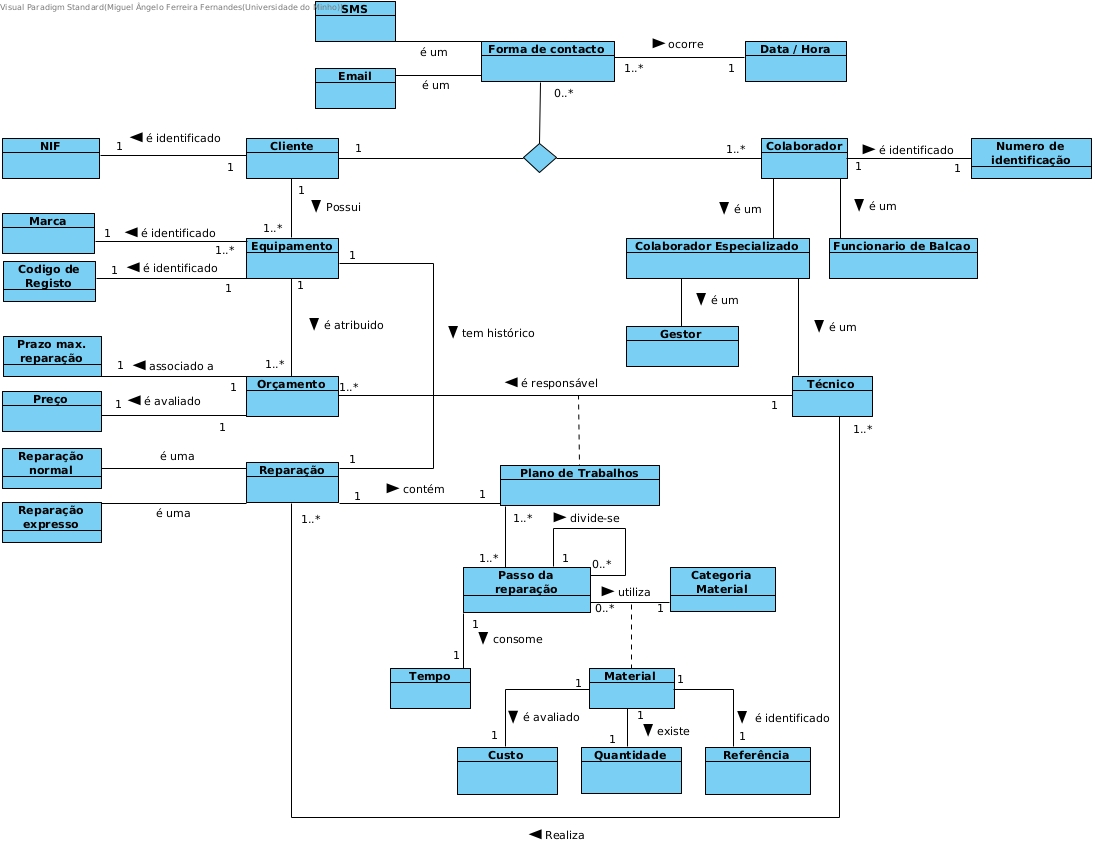
\includegraphics[scale=0.40]{Modeloinicial.jpg}
    \caption{Modelo de Domínio}
\end{figure}

\subsection{Modelo de Domínio Atual}

\begin{figure}[!ht]
    \centering
    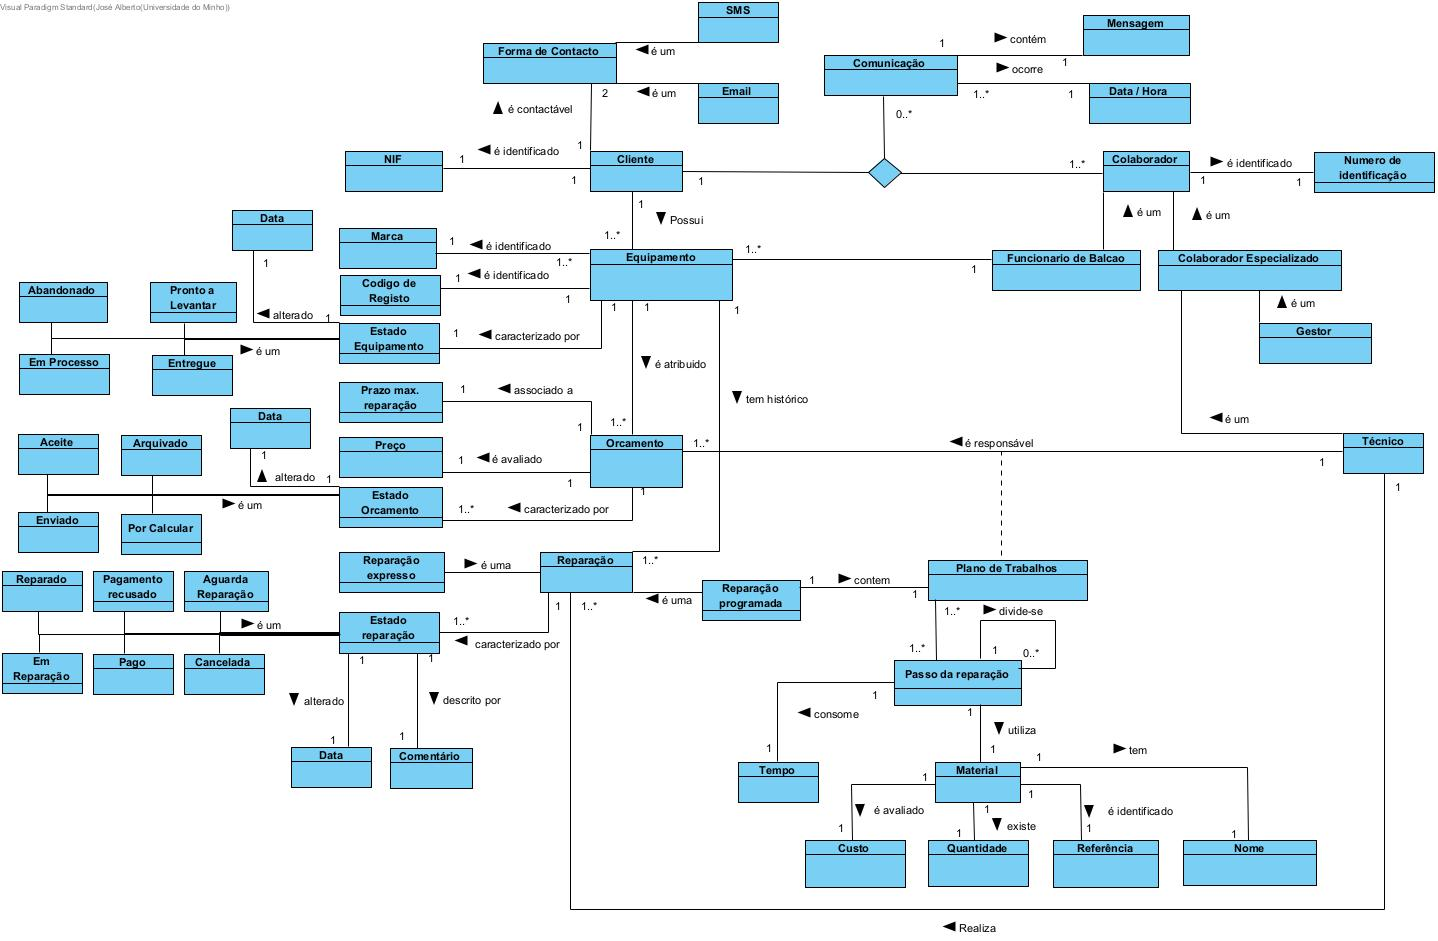
\includegraphics[scale=0.30]{ModeloDominio.jpg}
    \caption{Modelo de Domínio}
\end{figure}

\chapter{Modelação dos Requisitos Funcionais} \label{modelacao_req_funcionais}

A partir dos cenários (ver \ref{cenarios}) identificados pela equipa docente, 
foram identificados os seguintes \textit{use cases}:

\begin{itemize}
    \item Criar reparação expresso - \ref{criar_rep_expresso}
    \item Pedir orçamento - \ref{pedir_orcamento}
    \item Fazer orçamento - \ref{fazer_orcamento}
    \item Criar passo da Reparação - \ref{criar_passo_rep}
    \item Confirmar orçamento - \ref{confirmar_orcamento}
    \item Arquivar orçamento - \ref{arquivar_orcamento}
    \item Realizar reparação - \ref{realizar_rep}
    \item Realizar passo de reparação - \ref{realizar_passo_rep}
    \item Adicionar material - \ref{adicionar_material}
    \item Encomendar material - \ref{encomendar_material}
    \item Receber material - \ref{receber_material}
    \item Entregar equipamento - \ref{entregar_equipamento}
    \item Dar baixo do equipamento - \ref{dar_baixa_equipamento}
    \item Pedir reparação expresso - \ref{pedir_rep_xpress}
    \item Registar equipamento - \ref{registar_equipamento}
    \item Registar cliente - \ref{registar_cliente}
    \item Registar Colaborador - \ref{registar_colab}
    \item Autenticar Colaborador- \ref{autenticar_colab}
    \item Listar resumida do técnico - \ref{listagem_tecnico_resumida}
    \item Listar detalhada do técnico - \ref{listagem_tecnico_detalhada}
    \item Listar funcionário do balcão - \ref{listagem_func_balcao}
\end{itemize}
\section{Modelo de Use Cases}

\begin{figure}[!ht]
    \centering
    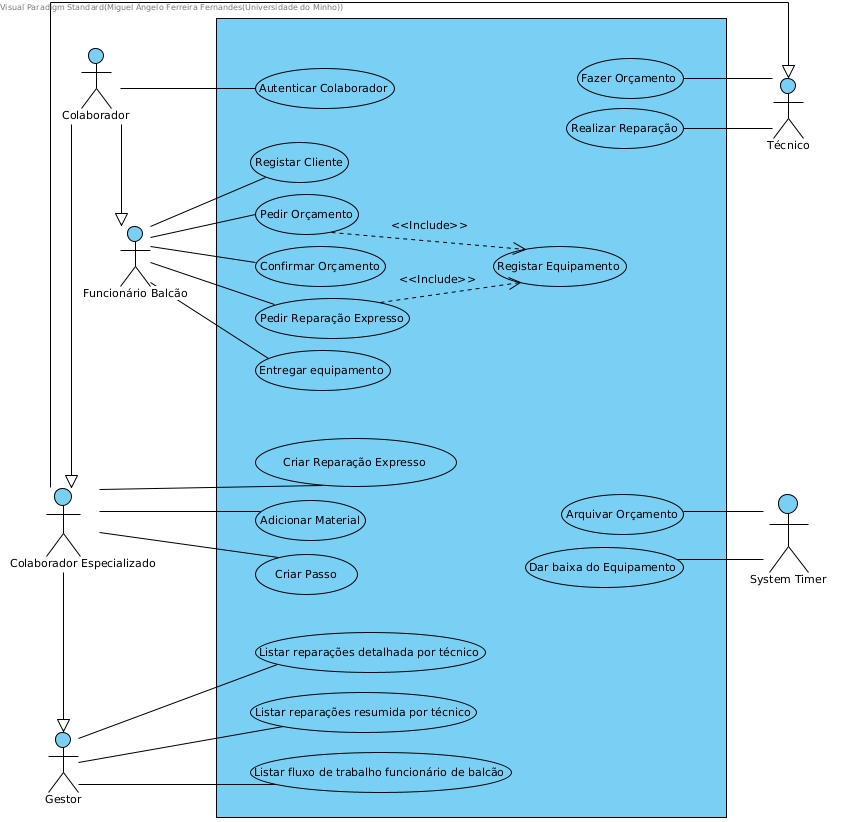
\includegraphics[scale=0.45]{dss-usecase.jpg}
    \caption{Diagrama de \textit{Use Case}}
\end{figure}

\subsection{Principais Diferenças com a Primeira Fase}

Em relação ao Diagrama de Use Cases desenvolvido, houve poucas alterações do que foi proposto na primeira fase do projeto.
Previamente, os casos de Uso \textbf{Dar Baixa do Equipamento} (Ver \ref{dar_baixa_equipamento}) e \textbf{Arquivar Orçamento} (Ver \ref{arquivar_orcamento})
seriam efetuadas pelo ator \textit{System Timer}. Contudo, após uma análise da aplicação e das dinâmicas exprimidas, entendeu-se como 
preferencial o \textbf{Gestor} efetuar estas funcionalidades, de modo a permitir visualizar os equipamentos que levaram baixa e os orçamentos que foram arquivados,
no momento em que o Gestor escolhe.
Foi retirado, então, o \textit{System Timer} como ator no diagrama de Use Cases.
Neste sentido, beneficia, também, a nível de implementação, não sendo necessário uma estratégia de criar o \textit{System Timer} dentro do sistema.

É necessário demarcar a presença dos casos de uso:
\begin{itemize}
    \item Adicionar Material
    \item Encomendar Material
    \item Receber Material
\end{itemize}

Apesar da sua implementação não ter sido realizada, no estado atual da aplicação, são apresentados para representar funcionalidades que seriam implementadas 
em iterações seguintes do sistema.
Estes casos de uso lidam com a manipulação de \textit{stocks} e, no tipo de projeto a realizar, foram caracterizadas como não necessárias apresentar 
nesta iteração do sistema. Adicionalmente, a exclusão do desenvolvimento destas funcionalidades facilitou a implementacaodo sistema.

\section{Especificação Use Cases}

\subsection{} \label{criar_rep_expresso}
\subfile{use_cases/usecase_criar-rep-xpress.tex}

\subsection{} \label{pedir_orcamento}
\subfile{use_cases/usecase_pedir-orcamento.tex}

\subsection{} \label{fazer_orcamento}
\subfile{use_cases/usecase_fazer-orcamento.tex}

\subsection{} \label{criar_passo_rep}
\subfile{use_cases/usecase_criar-passo.tex}

\subsection{} \label{confirmar_orcamento}
\subfile{use_cases/usecase_confirmar-orcamento.tex}

\subsection{} \label{arquivar_orcamento}
\subfile{use_cases/usecase_arquivar-orcamento.tex}

\subsection{} \label{realizar_rep}
\subfile{use_cases/usecase_realizar-reparacao.tex}

\subsection{} \label{realizar_passo_rep}
\subfile{use_cases/usecase_realizar-passo-reparacao.tex}

\subsection{} \label{adicionar_material}
\subfile{use_cases/usecase_adicionar-material.tex}

\subsection{} \label{encomendar_material}
\subfile{use_cases/usecase_encomendar-material.tex}

\subsection{} \label{receber_material}
\subfile{use_cases/usecase_receber-material.tex}

\subsection{} \label{entregar_equipamento}
\subfile{use_cases/usecase_entregar-equipamento.tex}

\subsection{} \label{dar_baixa_equipamento}
\subfile{use_cases/usecase_dar-baixa.tex}

\subsection{} \label{pedir_rep_xpress}
\subfile{use_cases/usecase_pedir-reparacao-expresso.tex}

\subsection{} \label{registar_equipamento}
\subfile{use_cases/usecase_registar-equipamento.tex}

\subsection{} \label{registar_cliente}
\subfile{use_cases/usecase_registar-cliente.tex}

\subsection{} \label{registar_colab}
\subfile{use_cases/usecase_registar-colaborador.tex}

\subsection{} \label{autenticar_colab}
\subfile{use_cases/usecase_autenticar-colaborador.tex}

\subsection{} \label{listagem_tecnico_resumida}
\subfile{use_cases/usecase_listar-tecnico-resumida.tex}

\subsection{} \label{listagem_tecnico_detalhada}
\subfile{use_cases/usecase_listar-tecnico-detalhada.tex}

\subsection{} \label{listagem_func_balcao}
\subfile{use_cases/usecase_listar-func-balcao.tex}

\chapter{Modelação Conceptual} \label{chap:modelacao_conceptual}

\section{Diagrama de Componentes} \label{sec:diagrama_componentes}
\subfile{model_funcional/diagrama_componentes.tex}

\section{Diagrama de Classes} \label{sec:diagrama_classe}

\subsection{SSClientes} 
Neste subsistema podem-se encontrar as funcionalidades relacionadas com os \textbf{Clientes}. 
Apesar de cada subsistema não estar intrinsecamente dependente de outros, estes não deixam de 
se relacionarem, como se pode verificar neste caso, com o SSReparacoes. Também é de salientar que neste
subsistema predomina uma arquitetura com agregação entre classes.


Aqui encontra-se, entre a classe Equipamento e Cliente, um caso de navegabilidade bidirecional, 
na medida a facilitar o acesso. É de salientar a atribuição de um estado ao equipamento, de maneira, a facilitar todo o processo da reparação, 
atribuíndo um ponto de situação ao mesmo e, também, a atribuição de uma forma de contacto ao cliente, de maneira a que este possa ser contactado quando necessário.


\subsubsection{GestClientesFacade}
Esta classe permite a gestão dos clientes e dos respetivos equipamentos associados, implementando a interface IGestClientes.

Analisando os métodos que esta classe implementa, identificou-se que, para melhorar a navegabilidade
e a \textit{performance} do sistema, será necessário que este tenha um conjunto de atributos, nomeadamente:
\begin{itemize}
    \item[clientes]{Mapa de clientes que pode ser acessido através do seu identificador, nif}
    \item[equipamentos]{Mapa de equipamentos que pode ser acessido através do seu ID} 
\end{itemize}

\begin{figure}[!ht]
    \centering
    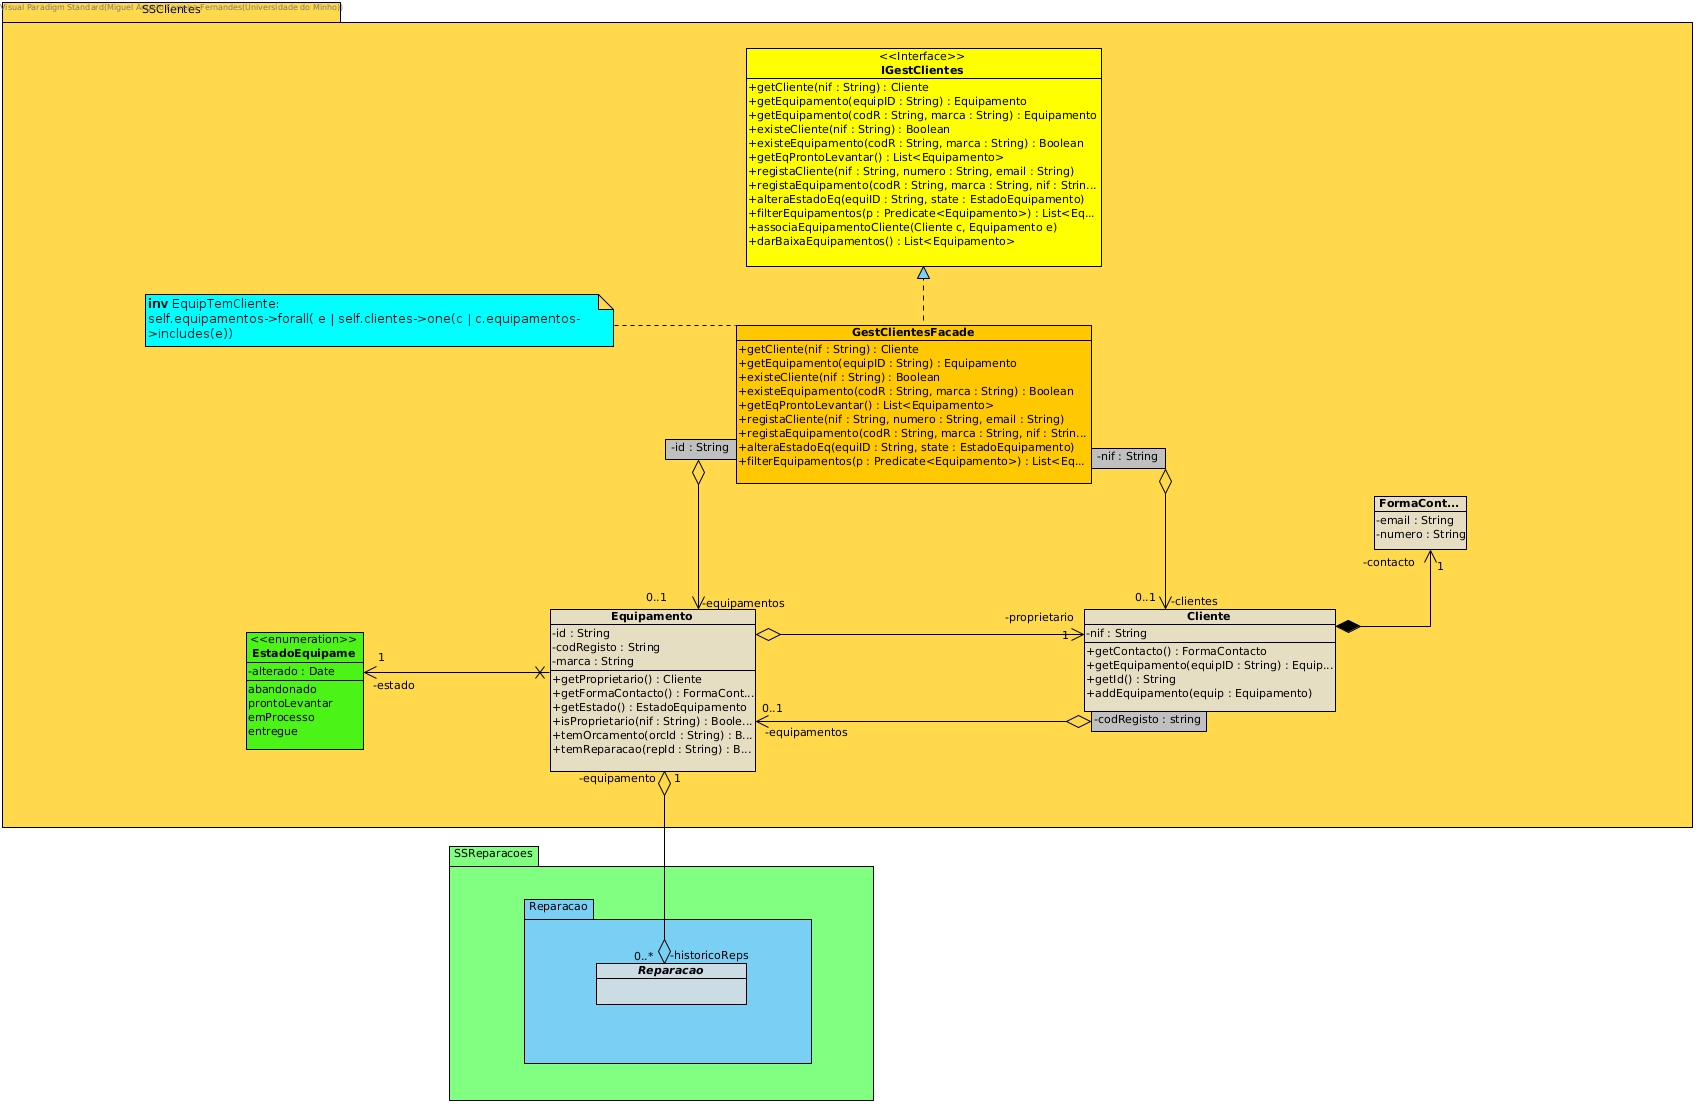
\includegraphics[scale=0.29]{SSClientes.jpg}
    \caption{SubSistema SSClientes}
\end{figure}

\subsection{SSColaboradores}
Neste subsistema podem encontrar-se as funcionalidades relacionadas com os \textbf{Colaboradores}.
Existem 2 tipos de colaboradores, nomeadamente:
\begin{itemize}
    \item [Colaborador]{Funcionário do Balcão}
    \item [Colaborador Especializado] {Técnico e Gestor}
\end{itemize}

Para facilitar todo o trabalho por parte do funcionário do balcão foi criado o \textit{package} Balcão, que é responsável pela gestão da
receção e entrega dos equipamentos guardando as respetivas datas, assim, é intuitivo a relação com o subsistema SSClientes, visto que,
a classe equipamento faz parte do mesmo.

Por outro lado, para facilitar toda a gestão de tempo e/ou disponibilidade por parte dos colaboradores especializados, nomeadamente, o Técnico, na realização das 
diversas reparações, foi criado um \textit{package} Agenda. 

O gestor, por sua vez, é responsável pelas listagens dos seus subordinados.

Também é de salientar que neste subsistema predomina uma arquitetura com composição entre classes.

\subsubsection{GestColaboradoresFacade}
Esta classe é responsável por toda a gestão dos colaboradores e funcionalidades, implementando a interface IGestColaboradores.

Analisando os métodos que esta classe implementa, identificou-se que, para melhorar a navegabilidade
e a \textit{performance} do sistema, será necessário que este tenha um conjunto de atributos, nomeadamente:
\begin{itemize}
    \item [balcao]
    \item [colabs]{Mapa de colaboradores que pode ser acessido através do seu ID}
    \item [agenda]
\end{itemize}

\begin{figure}[!ht]
    \centering
    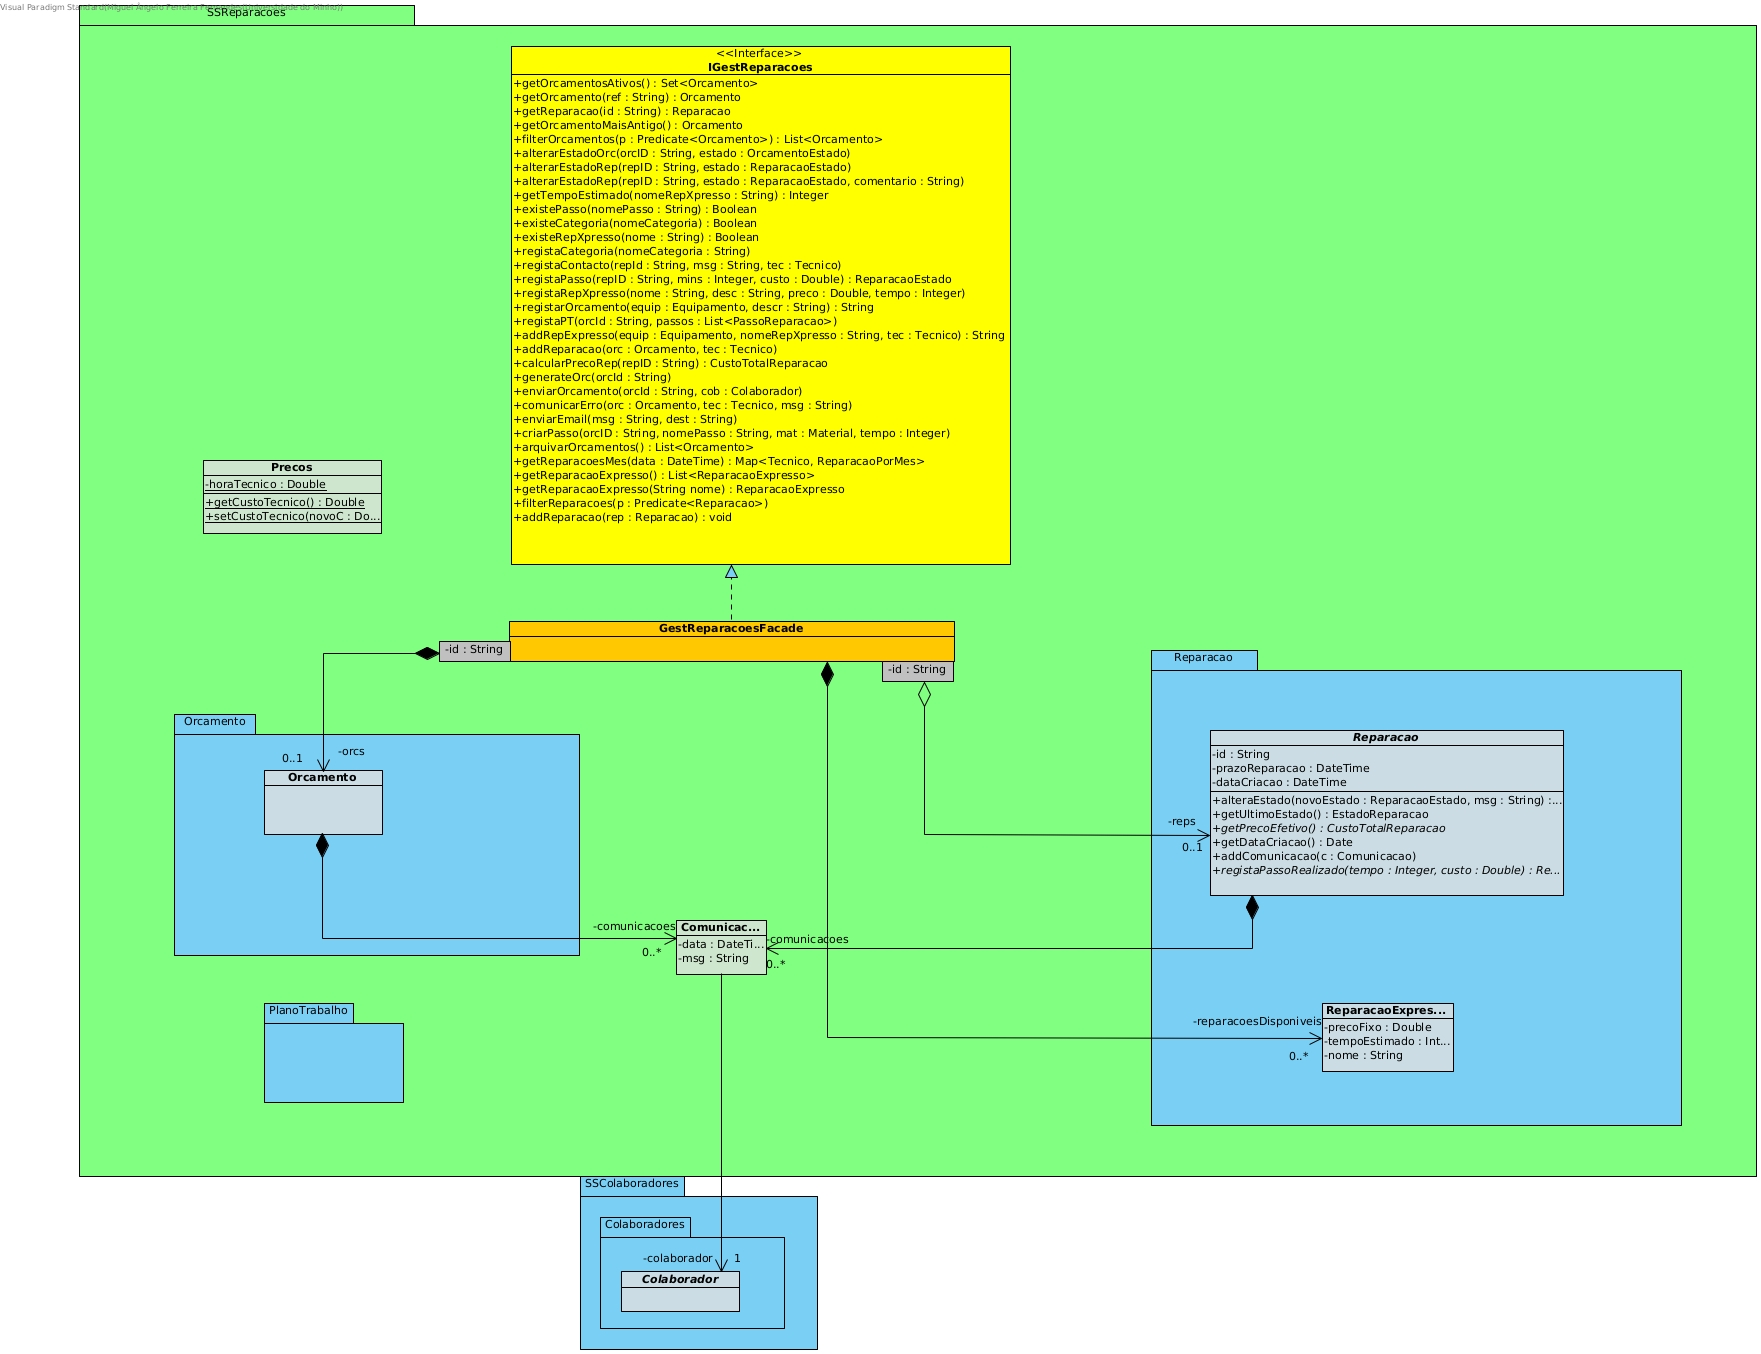
\includegraphics[scale=0.27]{SSReparacoesPackage.jpg}
    \caption{SubSistema SSReparacoes}
\end{figure}


\subfile{model_funcional/classe/diagrama_classes.tex}

\section{Diagramas de Sequência} \label{sec:diagrama_sequencia}
\subfile{model_funcional/diagrama_sequencia.tex}

\section{Diagrama de Package} \label{sec:diagrama_package}
\subfile{model_funcional/diagrama_package.tex}

\chapter{Implementação} \label{chap:implementacao}
\subfile{implementacao.tex}


\chapter{Considerações Finais}
Ao longo da realização da fase de análise de requisitos do projeto, houve a necessidade de utilizar conceitos
com os quais os elementos do grupo não estavam familiarizados.
A sua utilização obrigou a uma aprendizagem ativa, por forma a se conseguir dar resposta aos objetivos propostos.
Tal como qualquer instância de aprendizagem, houve dificuldades na sua implementação.
Em particular: familiarização da linguagem UML e \underline{capacidade de abstração} \underline{do problema}.
Esta última foi a mais difícil de ultrapassar, pois o grupo tendia a olhar para o modelo como sendo a realidade
e não uma representação abstrata da mesma.
A título exemplificativo, inicialmente foi definido um \textit{use case} que refletia todo um fluxo real
(desde que o cliente entra até que sai com o problema resolvido).
Posteriormente, através de estudo e acompanhamento da equipa docente, foi possível melhorar esta capacidade de abstração
e atingir um resultado final que o grupo acredita ir de encontro com os objetivos propostos.
Não obstante, o grupo ter atravessado algumas dificuldades, os resultados de aprendizagem acabaram por compensar.
Com a concretização desta fase, o grupo encontra-se mais capaz de modelar um problema utilizando a abstração necessária.

Apesar do grupo considerar que a solução a que chegou é suficiente e adequada, a sua falta de experiência
ao nível da conceção e implementação de soluções não lhe permite ser capaz de fazer a devida análise.
Por este motivo, o grupo tem consciência que se encontra perante um processo iterativo e que
na fase seguinte (modelação conceptual e implementação da solução), provavelmente, encontrará algumas dificuldades
em que será obrigado a fazer alterações da fase a que o presente relatório se refere.


%==========================================================================
% BEGIN LISTA DE SIGLAS E ACRÓNIMOS
%==========================================================================

%% Portuguese babel does not translate this environment
\renewcommand{\nomname}{Lista de Siglas e Acrónimos}

%% Text that can be shown before acronyms list
\renewcommand{\nompreamble}{}

%% acronyms
\nomenclature[01]{\textbf{NIF}}{Número de Idenficação Fiscal}
\nomenclature[02]{UC}{Unidade Curricular}
\nomenclature[03]{DSS}{Desenvolvimento de Sistemas de Software}
\nomenclature[04]{aplicação}{Sistema de Gestão para Centro de Reparação de Equipamento Eletrónico}

%% Show acronyms
\printnomenclature

%==========================================================================
% END LISTA DE SIGLAS E ACRÓNIMOS
%==========================================================================


%==========================================================================
% BEGIN ANEXOS
%==========================================================================

\addchap{Anexos}
\addsec{Anexo 1 - Cenários } \label{cenarios}
\subfile{scenarios/scenario_1.tex}
\subfile{scenarios/scenario_2.tex}
\subfile{scenarios/scenario_3.tex}
\subfile{scenarios/scenario_4.tex}
\subfile{scenarios/scenario_5.tex}

%==========================================================================
% END ANEXOS
%==========================================================================


\end{document}